%!TEX root = ../dynamics.tex
\section{Market Analysis}
\label{sec:market}
Finally, we study the demand vs supply on Amazon MTurk market place.
In this case, $Demand$ is defined as the number of new tasks posted on the platform by the requesters, in addition we compute the average reward of the posted tasks. Conversely, $Supply$ is defined as the workforce that the crowd is providing concretized as the number of tasks that got completed in a given time window, again we computed the average reward of the completed tasks.
An initial observation that we make that the strong weekly periodicity that the demand (requesters) exhibit reflected by the autocorrelation that we computed on the number of available HITs as reported by Amazon Mturk (See Figure \ref{fig:autocorrelation1}.
\begin{figure}[htbp]
	\centering
		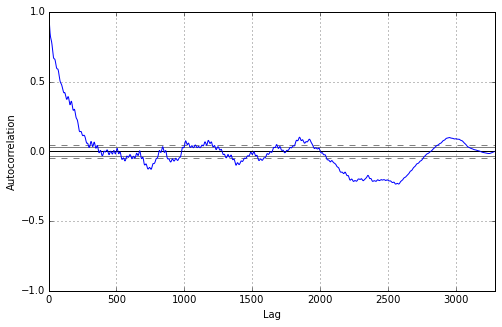
\includegraphics[width=0.5\textwidth]{figures/autocorrelation_plot}
	\caption{There is a significant memory for the market, as the autocorrelation of the 
number of HITS available (as reported by Amazon) lasts for approximately 7-10 days.}
	\label{fig:autocorrelation1}
\end{figure}

\subsection{Effect of New Tasks}
\begin{figure}[htbp]
	\centering
		
\includegraphics[width=0.5\textwidth]{figures/scattermatrix}
	\caption{Scatter matrix comparing the different parameters in the demand and supply.}
	\label{fig:scatter_matrix}
\end{figure}
\begin{figure}[htbp]
	\centering
		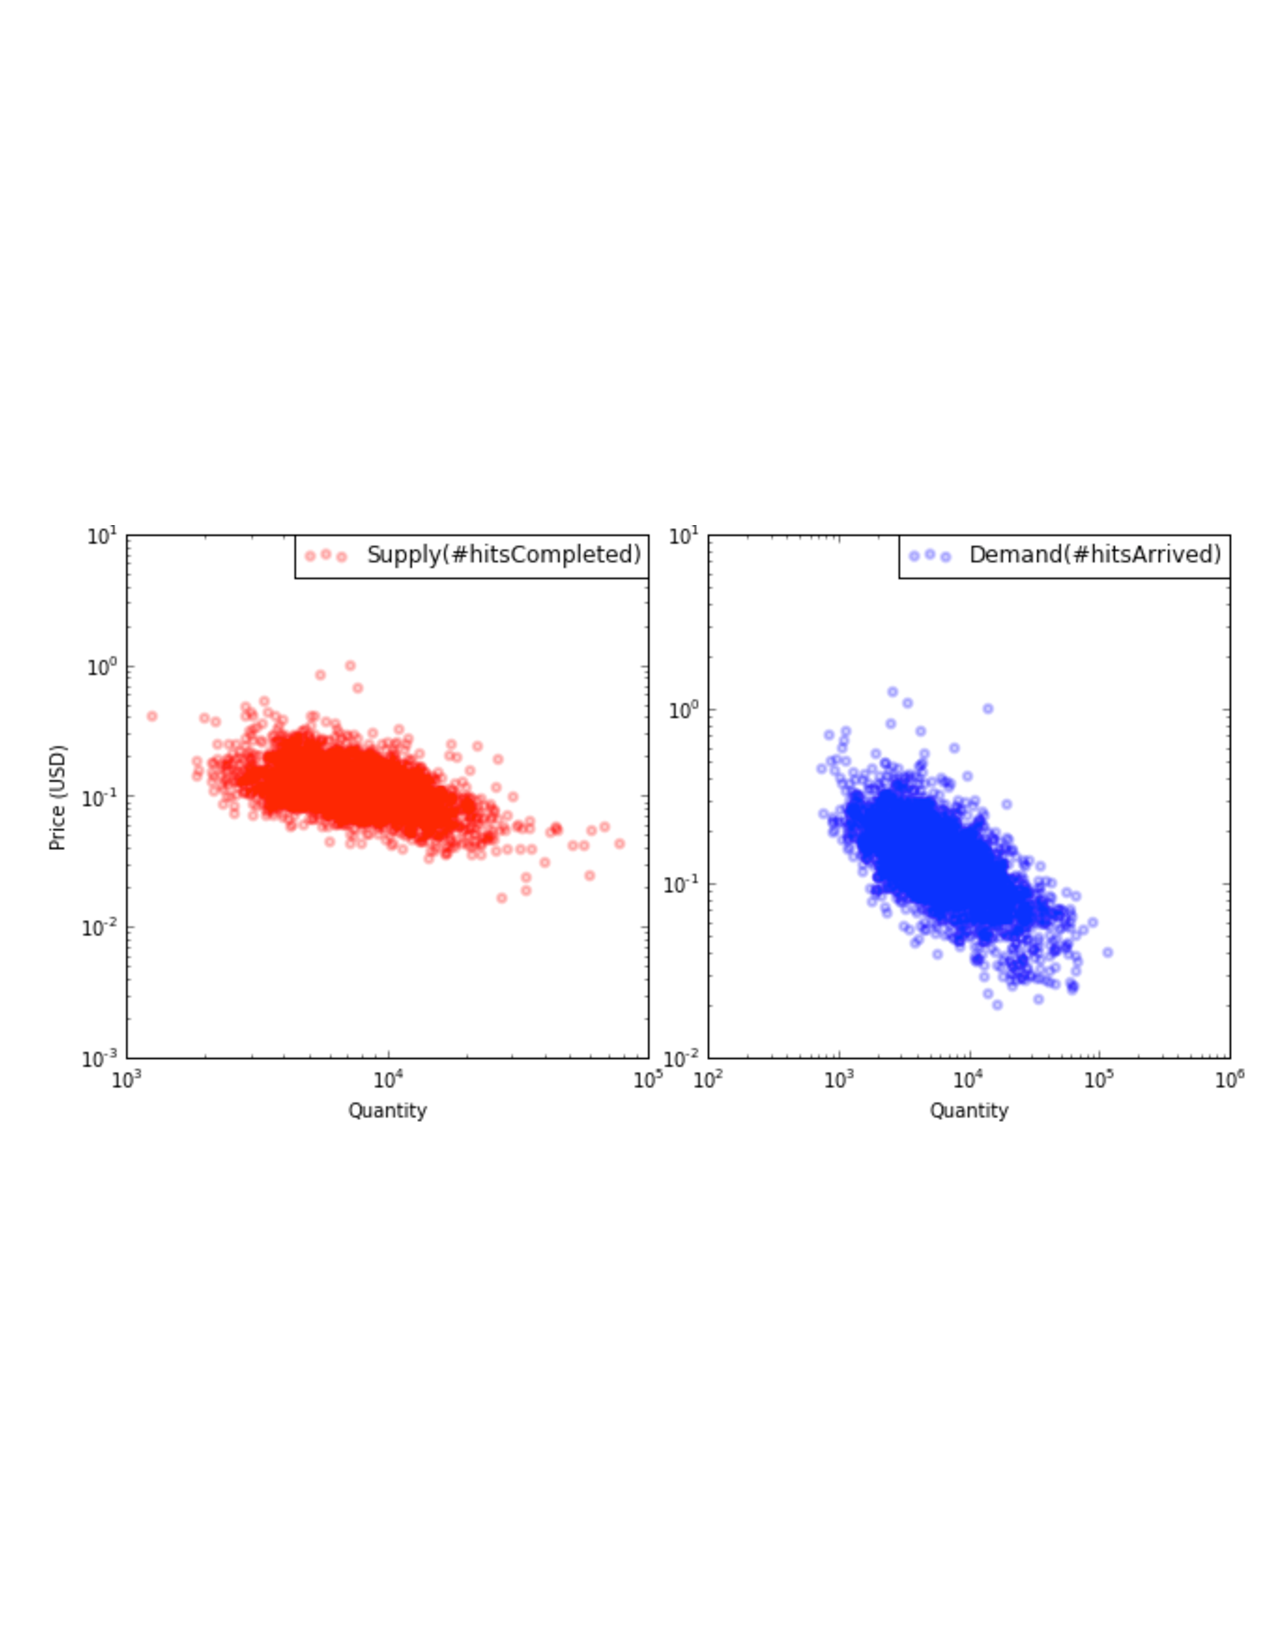
\includegraphics[width=0.5\textwidth]{figures/supply_demand}
	\caption{Demand and supply versus price.}
	\label{fig:dsup}
\end{figure}
In figure\ref{fig:scatter_matrix} we compare all the variables \{hitsArrived, avgRewardsArrived, hitsCompleted,avgRewardsCompleted\}. Among the observations that can be made is the correlation between the rewards completed and those arrived, and also the correlation between hits completed and those arrived. This suggests that the workers are sensitive to newly posted tasks, and that they are monitoring for new and fresh tasks, this supplements our finding in section\ref{sec:throughput} that $Start\_time$ is an important feature contributing to the throughput of a batch.
Figure \ref{fig:dsup}(a) shows a the usual relationship between demand and price, that is, the larger the demand the lower the price becomes. On the other hand Figure \ref{fig:dsup}(b) the supply doesn't match the typical supply curve (higher prices drive higher supply) instead the demand seems to be tied to the the supply (the number of new HITs posted), a possible explanation to that is the lack of biding mechanisms that the workers can leverage to drive prices up.

\subsection{Effect of New Workers}
\begin{figure}[htbp]
	\centering
		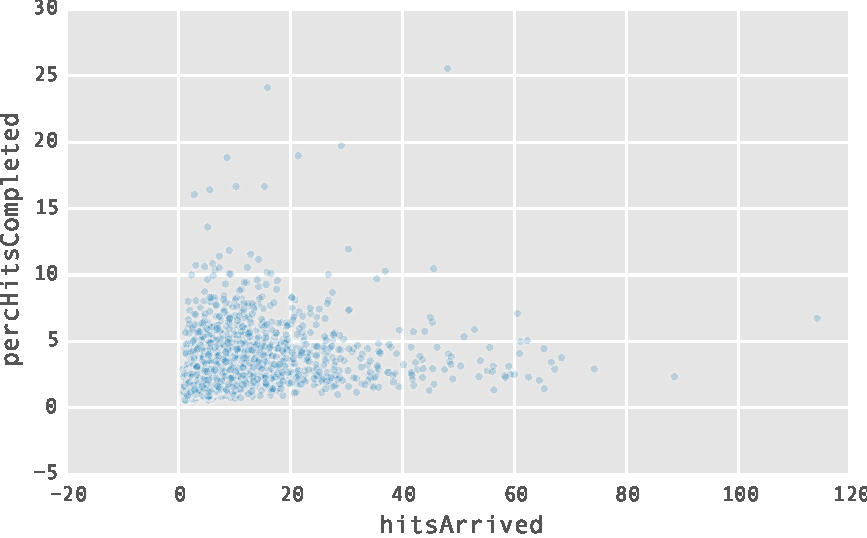
\includegraphics[width=0.5\textwidth]{figures/percHitsCompleted}
	\caption{The effect of new arrived HITs on the work provided supplied.}
	\label{fig:perc_hits_completed}
\end{figure}
Along the same lines, the results detailed in Figure\ref{fig:perc_hits_completed} indicate that as more HITs arrive, a higher percentage of the available work gets done. 
This clearly indicates that the arrival of new work also attracts new workers
in the market, who also seem to spillover to other tasks.

\subsection{Weekly Periodicity}
We computed the weekly moving average convergence/divergence (MACD) in Figure\ref{fig:mac} then we proceeded to run an autocorrelation to check whether there is some periodicity in the time series. Figure\ref{fig:autocorrelation2} shows that there is a strong weekly periodicity.
\begin{figure}[htbp]
	\centering
		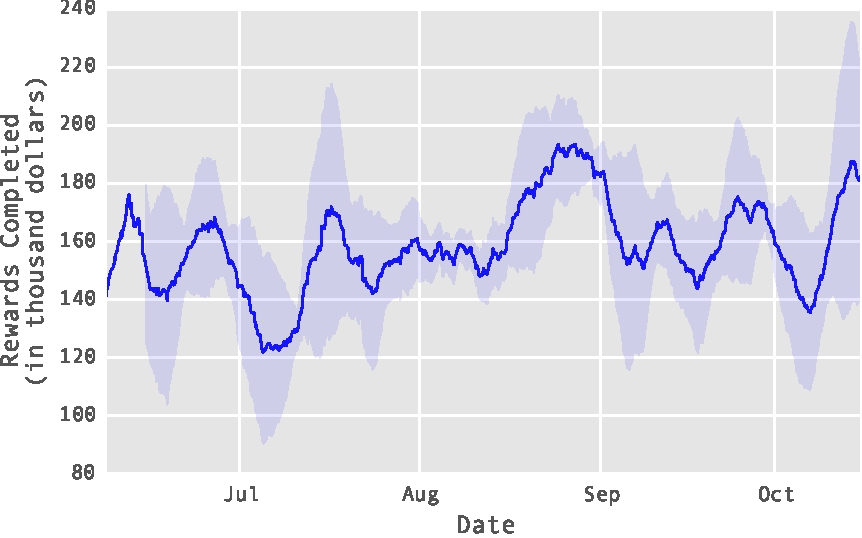
\includegraphics[width=0.5\textwidth]{figures/mac}
	\caption{Weekly Moving Average Convergence/Divergence (MACD) of the rewards completed.}
	\label{fig:mac}
\end{figure}
\begin{figure}[htbp]
	\centering
		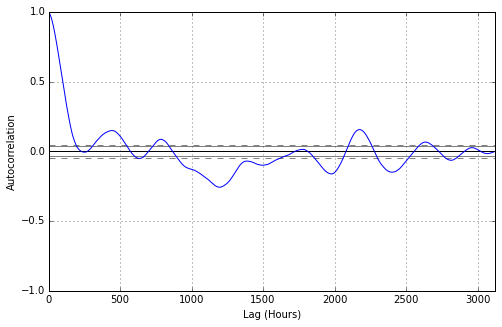
\includegraphics[width=0.5\textwidth]{figures/autocorrelation2}
	\caption{Autocorrelation computed on the weekly MACD.}
	\label{fig:autocorrelation2}
\end{figure}